\chapter{Body}
\section{Figure and Table}
In this section, we give some practical examples of inserting figure and table.

If you insert some figures, you should use \texttt{figure} environment. For example, you put the following code (Listing \ref{code:fig1}) and you can see Figure \ref{fig:itai}. 

% % \lstset command is used to config lstlisting environment, so it should be written in preamble.
\lstset{
  language={TeX},
  basicstyle={\footnotesize\ttfamily},
  keywordstyle={\color{blue}},
  morekeywords={begin, includegraphics, caption, label, subcaption, hline, multicolumn, DeclareAcronym },
  lineskip=-0.5pt
}
\begin{lstlisting}[caption=Example of Figure 1, label=code:fig1]
  \begin{figure}[htbp]
    \centering
    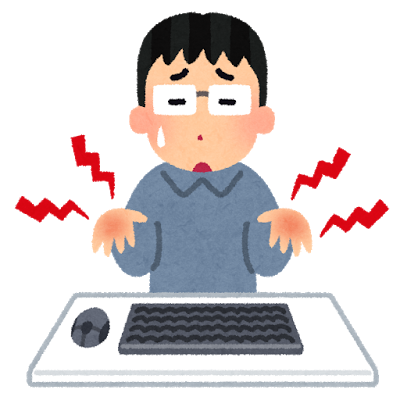
\includegraphics[scale=0.45]{./Figure/computer_keyboard_hand_itai.png}
    \caption{Illustration of you writing the master thesis}
    \label{fig:itai}
  \end{figure}
\end{lstlisting}

\begin{figure}[htbp]
  \centering
  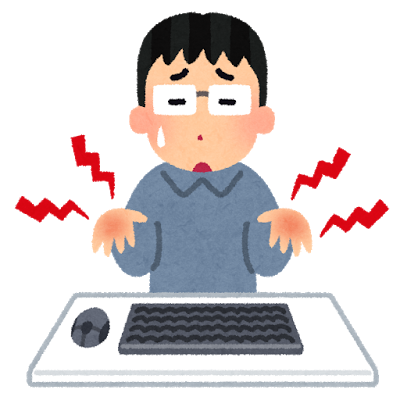
\includegraphics[scale=0.45]{./Figure/computer_keyboard_hand_itai.png}
  \caption{Illustration of you writing the master thesis}
  \label{fig:itai}
\end{figure}

Next example is a little more complex than previous one. If you arrange some figures horizontally, you put the following code (Listing \ref{code:fig2}) and you can see Figure \ref{fig:pc}. Moreover, using \verb+\ref{fig:desktop}+ or \verb+\subref{fig:desktop}+, you can get \ref{fig:desktop} or \subref{fig:desktop}.

\begin{lstlisting}[caption=Example of Figure 2, label=code:fig2]
  \begin{figure}[htbp]
    \begin{minipage}{0.48\hsize}
      \centering
      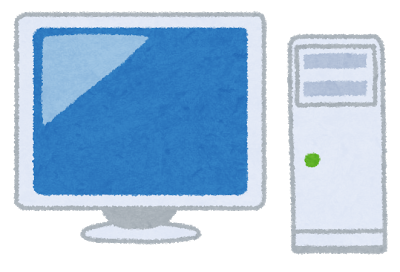
\includegraphics[scale=0.4]{./Figure/kaden_PC.png}
      \subcaption{Desktop PC}
      \label{fig:desktop}
    \end{minipage}
    \hfill
    \begin{minipage}{0.48\hsize}
      \centering
      
\includegraphics[scale=0.4]{./Figure/kaden_laptop.png}
      \subcaption{Laptop PC}
      \label{fig:laptop}
    \end{minipage}
    \caption{Two types of PC}
    \label{fig:pc}
  \end{figure}
\end{lstlisting}

\begin{figure}[htbp]
  \begin{minipage}{0.48\hsize}
    \centering
    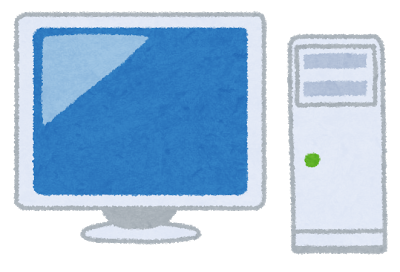
\includegraphics[scale=0.4]{./Figure/kaden_PC.png}
    \subcaption{Desktop PC}
    \label{fig:desktop}
  \end{minipage}
  \hfill
  \begin{minipage}{0.48\hsize}
    \centering
    
\includegraphics[scale=0.4]{./Figure/kaden_laptop.png}
    \subcaption{Laptop PC}
    \label{fig:laptop}
  \end{minipage}
  \caption{Two types of PC}
  \label{fig:pc}
\end{figure}

If you insert some tables, you should use \texttt{table} environment. For example, you put the following code (Listing \ref{code:table1}) and you can see Table \ref{table:1}. 

\begin{lstlisting}[caption=Example of Table 1, label=code:table1]
  \begin{table}
    \centering
    \caption{Example of table}
    \label{table:1}
    \begin{tabular}{c|cc|c}
      Name & Price & Number & Subtotal \\
      \hline
      Apple  & 130 & 3 & 390 \\
      Banana &  60 & 8 & 480 \\
      Orange & 100 & 5 & 500 \\
      \hline
      \multicolumn{3}{r|}{Total amount} & 1370
    \end{tabular}
  \end{table}
\end{lstlisting}

\begin{table}[htbp]
  \centering
  \caption{Example of table}
  \label{table:1}
  \begin{tabular}{c|cc|c}
    Name & Price & Number & Subtotal \\
    \hline
    Apple  & 130 & 3 & 390 \\
    Banana &  60 & 8 & 480 \\
    Orange & 100 & 5 & 500 \\
    \hline
    \multicolumn{3}{r|}{Total amount} & 1370
  \end{tabular}
\end{table}

\section{Citation}
In this section, we give some examples of citation. If you cite something from books or papers, you must append references in your paper. Using \texttt{.bib} file is convenient to manage references because \texttt{.bib} file format of papers has already been made by web service such as google scholar and IEEE Xplore Digital Library.

For example, if you cite a book named ``Citation example from a book'', you put \TeX\, command \verb+\cite{book1}+ and get the following \cite{book1}. Similarly, you cite 78 page of a paper named ``Citation example from a paper'', you put \verb+\cite[p. 78]{paper1}+ and get \cite[p. 78]{paper1}.

\section{Abbreviations and Symbols}
In this section, we introduce an convenient package named \texttt{acro} for abbreviations and symbols. If you show lists of either abbreviations, symbols or both, you should use this package. 

Listings \ref{code:acro1} and \ref{code:acro2} are example codes of an abbreviation and a symbol respectively. \texttt{short} field of abbreviations is the short form of a word, and \texttt{long} field is the long form. However, \texttt{short} field of symbols should be set a symbol, and \texttt{long} field should be written description of the symbol.

\begin{lstlisting}[caption=Example of a definition for an abbreviation, label=code:acro1]
  \DeclareAcronym{pc}{
    short = PC ,
    long  = Personal Computer ,
    class = abbrev
  }
\end{lstlisting}

\begin{lstlisting}[caption=Example of a definition for a symbol, label=code:acro2]
  \DeclareAcronym{A}{
    short = $\bm{A}$ ,
    long  = Matrix ,
    sort  = A ,
    class = nomencl
  }
\end{lstlisting}

We can define other words by similar codes, and should make up the definitions into a file (e.g., \texttt{./Chapter/Acronym.tex}). If you put \verb+\ac{ws}+ and \verb+\acs{A}+, you get \ac{ws} and \acs{A} respectively. Another example of output is the following. In this example, we called \verb+\ac{ws}+ again, so we obtain a different output than before. On the other hand, \verb+\acs{A}+ outputs same result because \verb+\acs{}+ command always outputs the short format of abbreviations and symbols.

\begin{screen}
\ac{ws}, \ac{pc} and \ac{uoa} are abbreviations whereas \acs{A}, \acs{a} and \acs{r} are part of the symbols.
\end{screen}
